\section{Extra\c{c}\~ao de Informa\c{c}\~ao}
	\begin{frame}
		\frametitle{\huge Extra\c{c}\~ao de Informa\c{c}\~ao}
		\begin{block}{\Large O que �?}
			\begin{itemize}
				\item A tarefa de identificar os fragmentos espec\'ificos de um \'unico documento que constituem o seu n\'ucleo sem\^antico
				\begin{itemize}
					\item Ex.: Relat\'orio de Clima e Tempo \Rightarrow  datas, temperaturas, locais.
				\end{itemize}
			\end{itemize}
		\end{block}		

	\end{frame}
	
	\begin{frame}
		\frametitle{MUC - Message Understanding Conference}			
		\begin{table}[htbp]
		  %\caption{Confer�ncias e seus temas}
		  \centering
		  \footnotesize
		  %\scriptsize
		  %\tiny
		    \begin{tabular}{cccc}
			    \addlinespace
			    \toprule
			    {\bf Confer�ncia} & {\bf Ano} & {\bf Fonte de Texto} & {\bf T�pico(Dominio)} \\
			    \midrule
			    MUC-1 & 1987 & Artigos Militares & Opera��es de fuga\\
			    MUC-2 & 1989 & Artigos Militares & Opera��es de fuga\\
			    MUC-3 & 1991 & Artigos de Jornais & Atividades Terroristas \\% na Am�rica Latina \\
			    MUC-4 & 1992 & Artigos de Jornais & Atividades Terroristas \\ %na Am�rica Latina \\
			    MUC-5 & 1993 & Artigos de Jornais & Corporate Joint Ventures\\
			    MUC-6 & 1995 & Artigos de Jornais & Negotiation of Labor Disputes \\
			    MUC-7 & 1997 & Artigos de Jornais & Acidente de avi�es \\
			    \bottomrule
		    \end{tabular}
		  \label{tab:MUC}
		\end{table}
		
	\end{frame}
	
	\begin{frame}
		\frametitle{\huge Tipos de Dados}
		\framesubtitle{\Large Documentos Livre}
			\begin{figure}[htb]
				\begin{center}				
					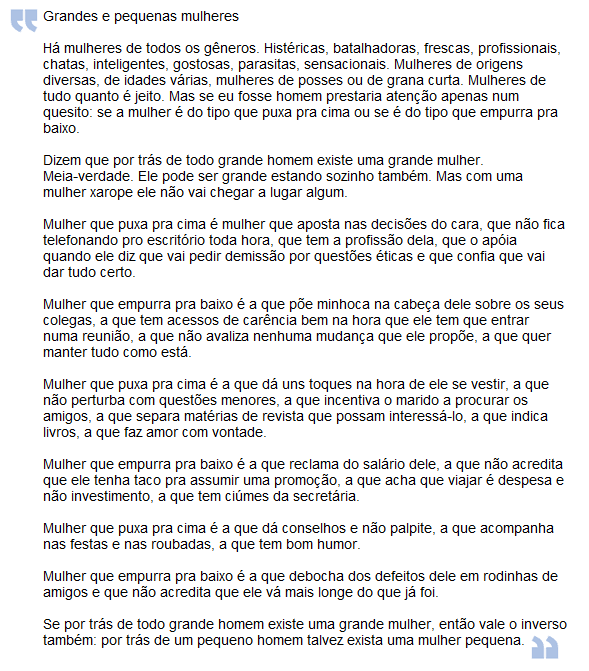
\includegraphics[scale=0.5]{./figuras/texto.png}				
				\end{center}
			\end{figure}		
	\end{frame}
	
	\begin{frame}
		\frametitle{\huge Tipos de Dados}
		\framesubtitle{\Large Documentos Semi-Estruturado}
			\begin{figure}[htb]
				\begin{center}				
					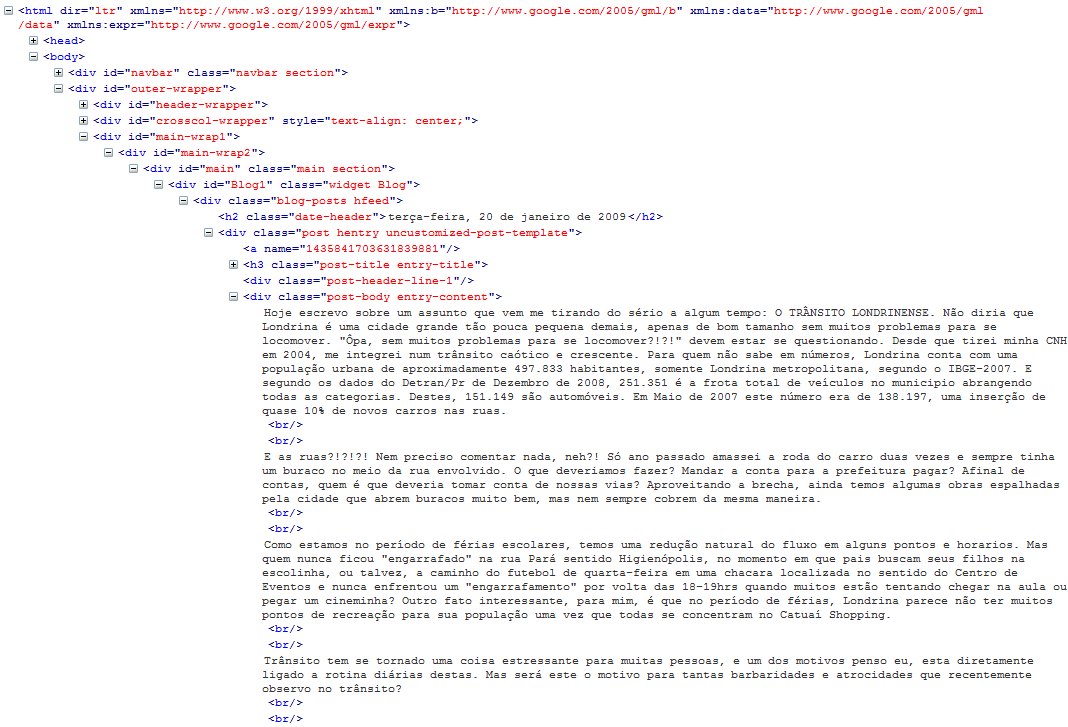
\includegraphics[scale=0.5]{./figuras/html.png}				
				\end{center}
			\end{figure}
	\end{frame}
	
	\begin{frame}
		\frametitle{\huge Tipos de Dados}
		\framesubtitle{\Large Documentos Estruturado} 
			\begin{figure}[htb]
				\begin{center}				
					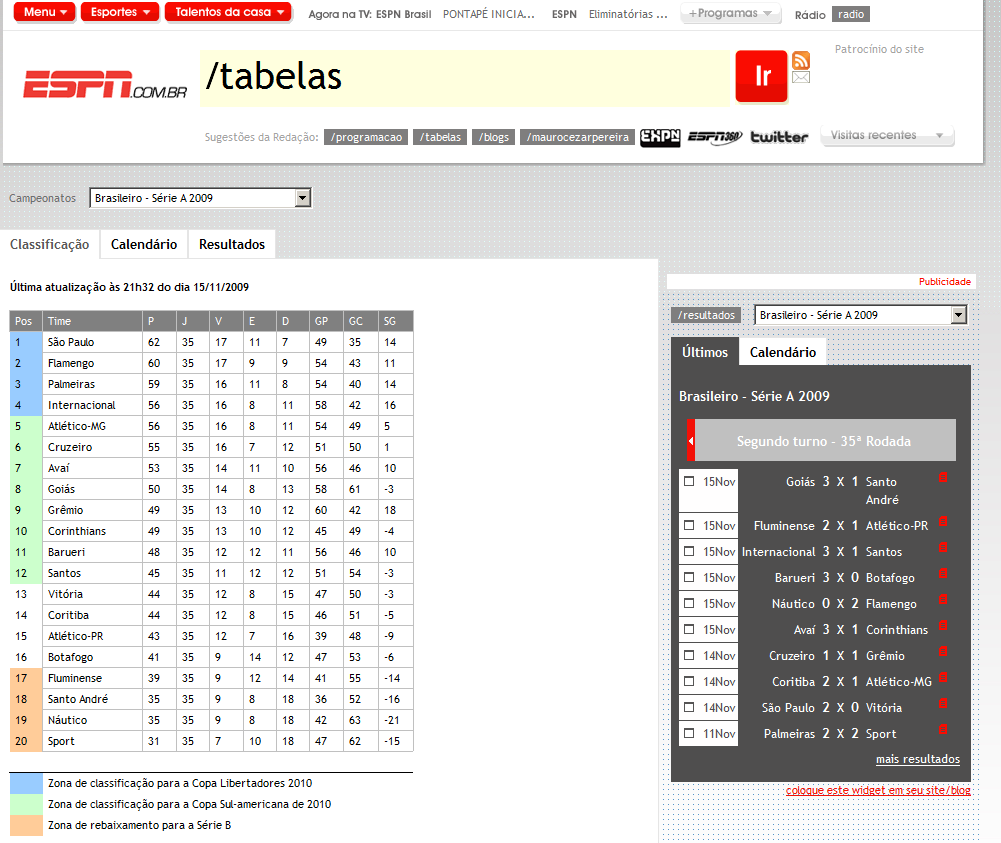
\includegraphics[scale=0.6]{./figuras/tabela.png}
				\end{center}
			\end{figure}		
	\end{frame}
	
	\begin{frame}
		\frametitle{\huge Extra\c{c}\~ao de Informa\c{c}\~ao}	
		\framesubtitle{\Large FLUXO GERAL}			
			\begin{figure}[htb]
				\begin{center}				
					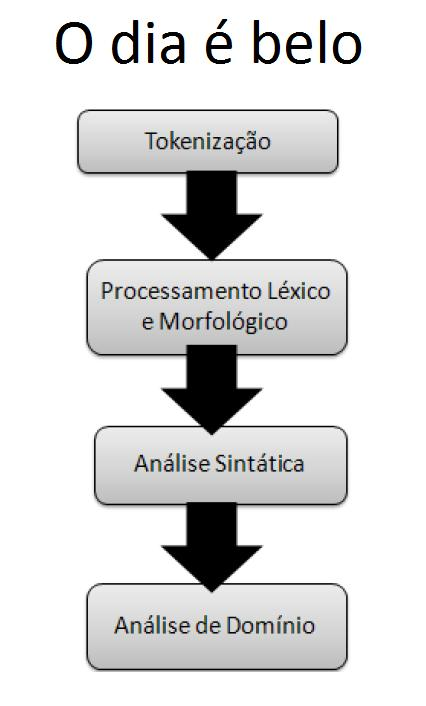
\includegraphics[scale=0.4]{./figuras/processo00.jpg}				
				\end{center}				
			\end{figure}
	\end{frame}
	
	\begin{frame}
		\frametitle{\huge Extra\c{c}\~ao de Informa\c{c}\~ao}	
		\framesubtitle{\Large FLUXO GERAL - Tokeniza��o}
			\begin{figure}[htb]
				\begin{center}				
					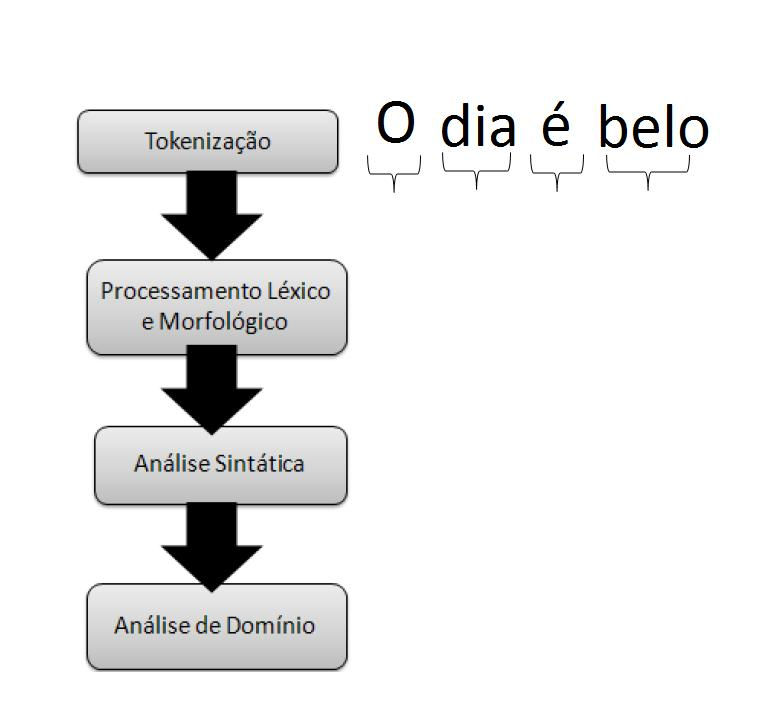
\includegraphics[scale=0.4]{./figuras/processo01.jpg}				
				\end{center}				
			\end{figure}
	\end{frame}

	\begin{frame}
		\frametitle{\huge Extra\c{c}\~ao de Informa\c{c}\~ao}	
		\framesubtitle{\Large FLUXO GERAL - Processamento Morfol�gico e L�xico}		
			\begin{figure}[htb]
				\begin{center}				
					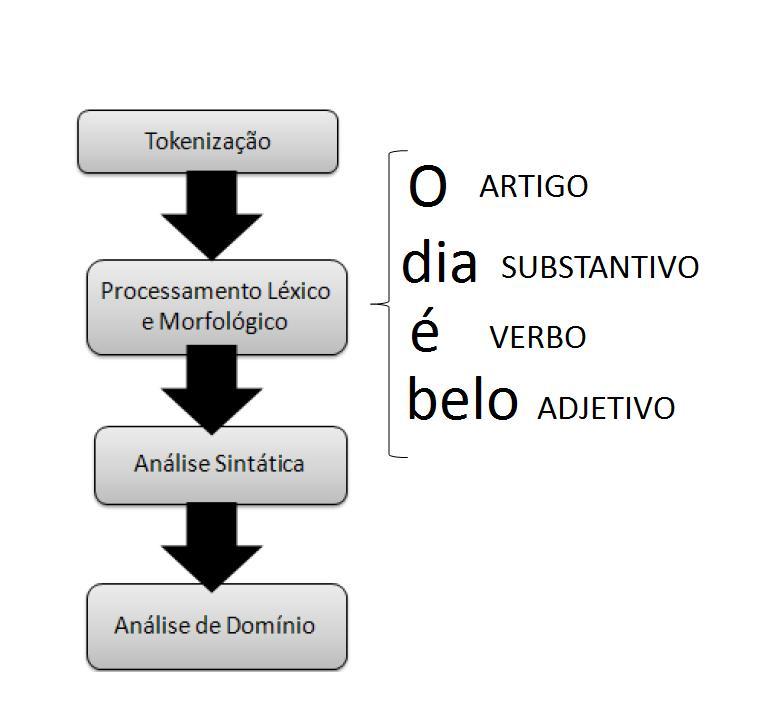
\includegraphics[scale=0.4]{./figuras/processo02.jpg}				
				\end{center}				
			\end{figure}
	\end{frame}
	
	\begin{frame}
		\frametitle{\huge Extra\c{c}\~ao de Informa\c{c}\~ao}	
		\framesubtitle{\Large FLUXO GERAL - Processamento Sint�tico}
			\begin{figure}[htb]
				\begin{center}				
					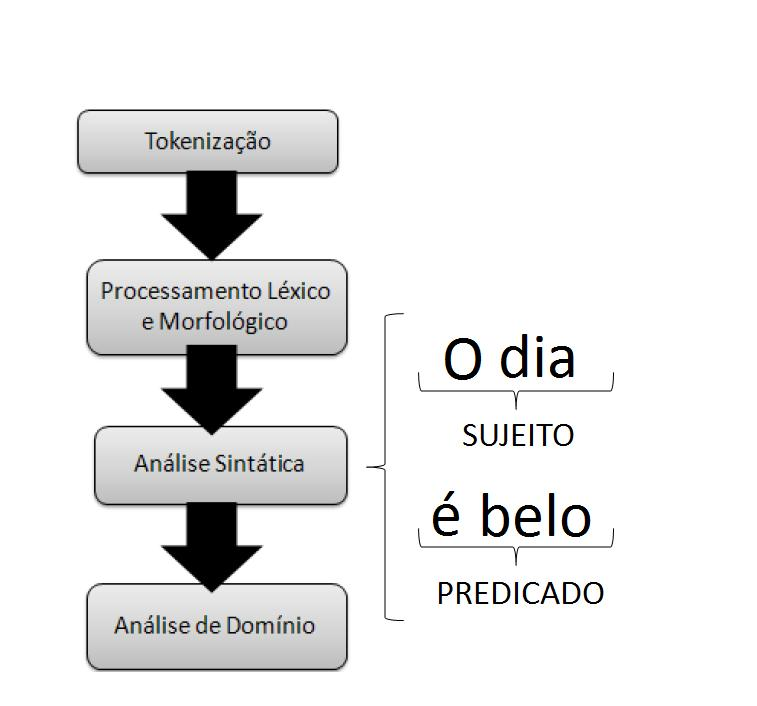
\includegraphics[scale=0.4]{./figuras/processo03.jpg}				
				\end{center}				
			\end{figure}
	\end{frame}
	
	\begin{frame}
		\frametitle{\huge Extra\c{c}\~ao de Informa\c{c}\~ao}	
		\framesubtitle{\Large FLUXO GERAL - An�lise de Dom�nio}		
			\begin{figure}[htb]
				\begin{center}				
					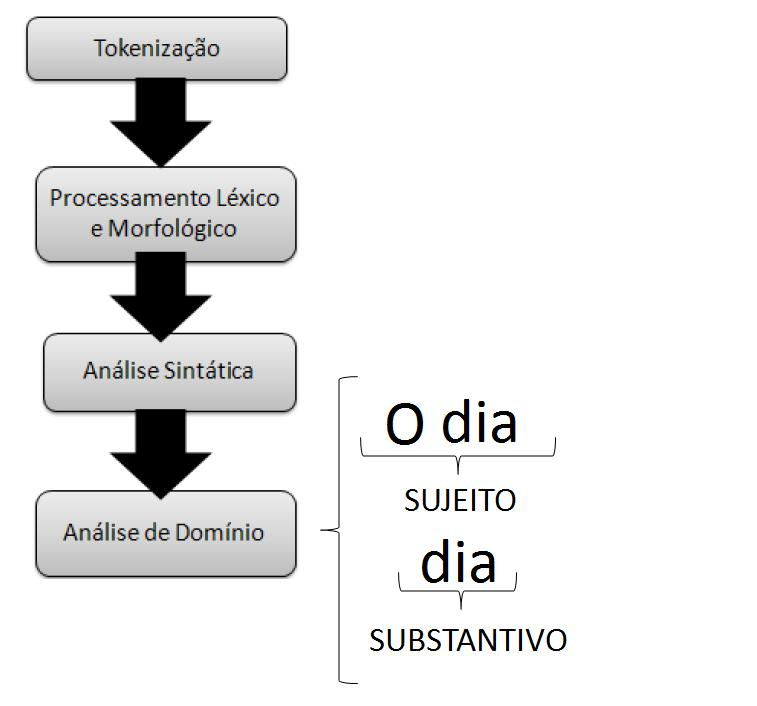
\includegraphics[scale=0.4]{./figuras/processo04.jpg}				
				\end{center}				
			\end{figure}
	\end{frame}
	
	\begin{frame}
		\frametitle{\huge Extra\c{c}\~ao de Informa\c{c}\~ao}	
		\framesubtitle{\Large AVALIA\c{C}\~AO}		
			\begin{figure}[htb]
				\begin{center}				
					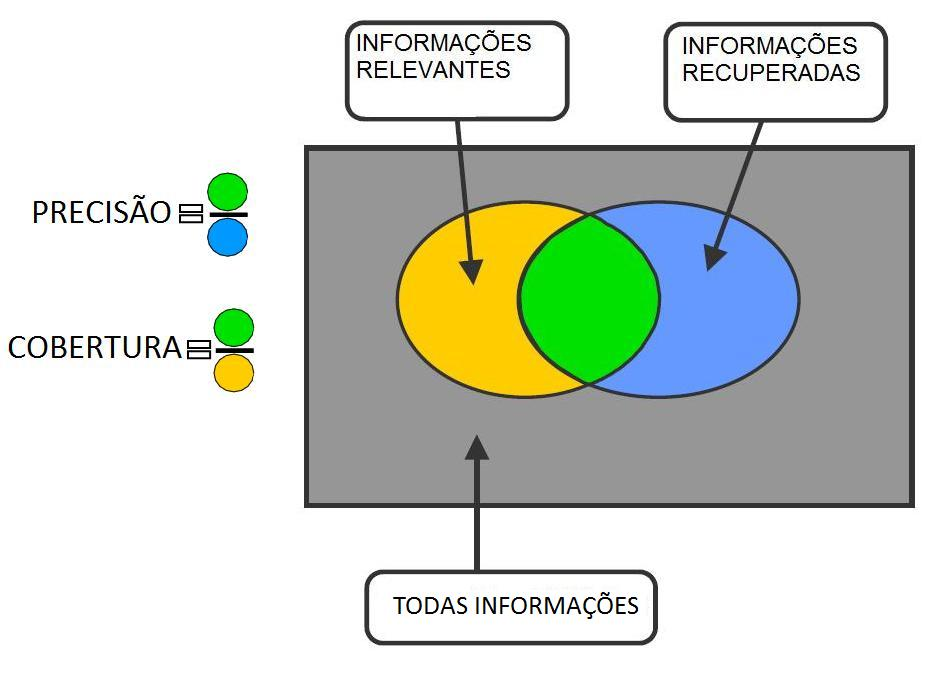
\includegraphics[scale=0.4]{./figuras/avaliacao01.jpg}
				\end{center}				
			\end{figure}
	\end{frame}